\section{真实生态中的技能}
\label{sec:insight}

\begin{figure*}[t]
  \centering
  \setlength{\abovecaptionskip}{0pt}
  \setlength{\belowcaptionskip}{-8pt}
  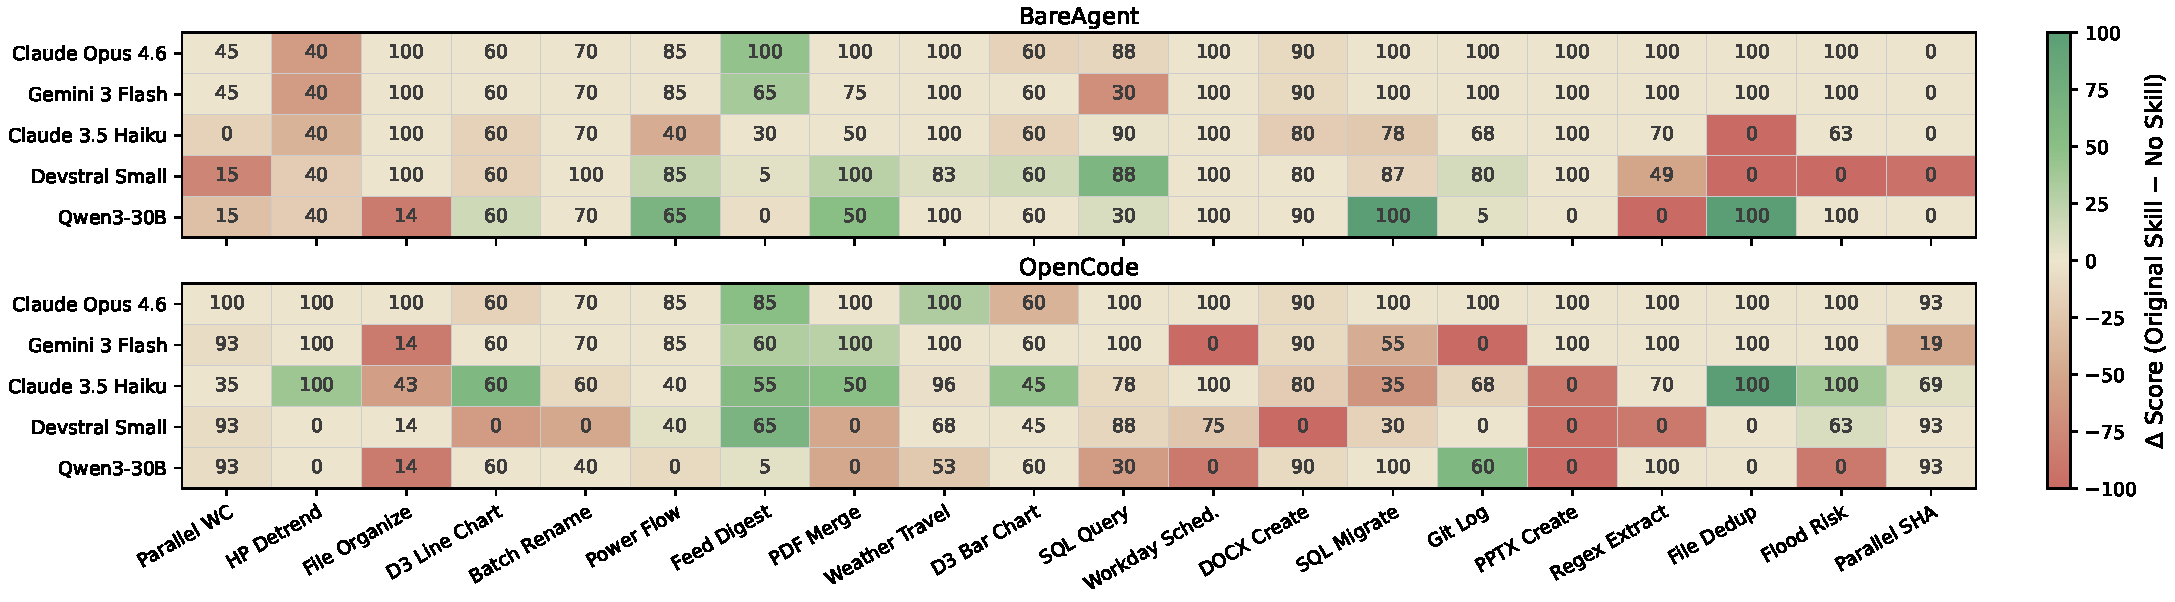
\includegraphics[width=\textwidth]{figures/m2_cross_harness_heatmap.pdf}
  \caption{不同模型与代理框架上的技能性能。列表示任务，行表示模型，每幅子图对应一个代理框架。单元格颜色表示相对于无技能基线的分数变化，单元格标签给出任务的绝对分数。模型身份与代理框架选择都会显著影响结果。}
  \label{fig:m2_heatmap}
\end{figure*}

本节首先介绍技能、使用技能的代理，以及技能在实践中的调用方式。
我们从两个主要分发平台收集了超过 110,000 个技能，
以大规模视角研究技能生态：
clawhub.ai~\cite{clawhub}（28,990 个技能）与 skills.sh~\cite{skillssh}（89,280 个技能）。
在这一生态分析的基础上，我们进一步开展实验，
识别当前技能使用中的具体问题。

\subsection{技能定义}
\label{sec:back:skills}

\emph{技能}是一种可分发、自包含的知识包，
用于增强 AI 代理处理某类特定任务的能力~\cite{claude-agent-skills, agentskills-spec}。
技能既可以引入基础模型原本不具备的知识，
也可以在模型已有相关能力但本会即兴处理时，约束模型遵循规定的工作流。
例如，一个 PDF 处理技能~\cite{anthropic-skills-repo} 会教模型如何使用 pdfplumber 提取表格，
同时也约束模型在合并 PDF 文件时使用 pypdf，而不是已弃用的 PyPDF2。

一个技能通常定义在包含三层结构的文件中：
（1）\emph{元数据}---名称、描述和触发条件，
使代理运行时能够自动发现并选择技能；
（2）\emph{指令}---技能主体，以自然语言编码
多步工作流、工具引用及其他任务专用指导；以及
（3）\emph{随附资源}---存储在配套文件中的脚本、参考资料与模板。

这一结构使技能区别于临时的提示词片段。
元数据使技能成为可发现、可选择的单元，令代理运行时能够自动把任务与适用技能匹配，而不必
手工拼装提示词~\cite{claude-code-skills}。
与微调相比，技能无需修改权重，
完全可以在提示词层面运行~\cite{ouyang2022training, liu2021pretrain}，因而分发轻量且易于组合。
多个代理平台已经趋同于这一抽象~\cite{claude-code-skills, cursor-skills, openai-codex-cli, agentskills-spec, antigravity-skills, coze-skills}，现有工具也已支持基础的技能编写、管理与优化。

\subsection{LLM 代理与代理框架}
\label{sec:back:harness}

LLM 代理在 ReAct 循环~\cite{yao2023react} 中工作。它接收任务，推理
下一步行动，发起工具调用（读取文件、运行命令、请求 API）~\cite{schick2023toolformer, openai2023functioncalling}，观察结果，然后再次推理。
这一循环会不断重复，直至任务完成。

代理并不直接与外部世界交互。
它运行在\emph{代理框架}之内；该运行时框架位于模型与操作环境之间~\cite{wu2023autogen, langgraph}。
代理框架负责管理 LLM API 连接、注册代理可调用的工具、分派这些调用，
并控制对话历史中有多少内容能够装入上下文窗口。
Claude Code~\cite{claudecode}、OpenCode~\cite{opencode} 和 OpenClaw~\cite{openclaw} 都是广泛使用的代理框架。

代理框架之间存在会影响技能的差异~\cite{google-a2a}。
有些框架提供丰富的文件系统与网络搜索工具，
另一些则只公开基本的读、写和 shell 执行操作。
有些框架可以生成彼此独立、并发工作的子代理，
另一些则只支持顺序执行。
这些差异会直接影响技能指令能否得到执行。

\subsection{技能特征分析}
\label{sec:insight:analysis}

\heading{生态规模与分布。}
技能生态规模庞大，但分布并不均衡。
图~\ref{fig:skill_distribution} 展示了两个平台上的下载次数。
在 skills.sh 上，89,280 个技能中有 89\% 的下载次数少于 86，
只有少数头部技能达到 $10^4$--$10^6$ 次。
clawhub.ai 也呈现类似的长尾形态，峰值约为 $10^2$--$10^3$ 次下载。
两个平台合计存在超过 118,000 个技能，但其中绝大多数很少被使用。
\begin{figure}[t]
  \centering
  \setlength{\abovecaptionskip}{0pt}
  \setlength{\belowcaptionskip}{-10pt}
  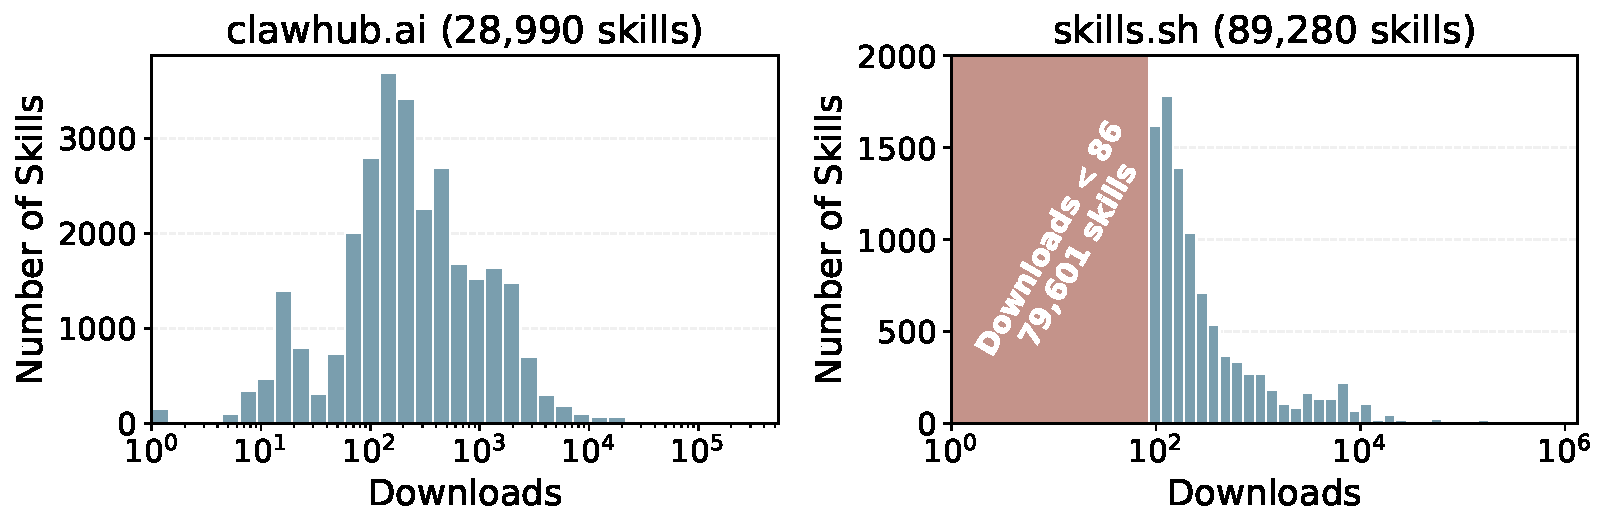
\includegraphics[width=\columnwidth]{figures/skill_download_distribution.pdf}
  \caption{clawhub.ai 与 skills.sh 上的技能下载分布。两个平台都呈现长尾分布。}
  \label{fig:skill_distribution}
\end{figure}

\heading{技能分类。}
技能为代理提供的内容差异很大。
我们借助 LLM 分析，将下载次数超过 100 的 15,063 个技能
按照技能最强调的方面分为三类：工具参考（52\%）、
流程指导（28\%）和内容生成（20\%）。

\emph{工具参考型技能}教模型如何操作特定工具、API 或 CLI。
它们本质上是加载到代理上下文中的使用文档。
一个典型例子是说明如何使用 Python 合并、拆分和处理 PDF 文件的技能。

\emph{流程型技能}规定执行任务时应遵循的逐步工作流与推理策略。
一个典型例子是强制采用四阶段流程的调试技能：复现故障、追踪根因、
施加针对性修复，并通过测试验证修复。

\emph{生成型技能}要求模型生成内容、代码、文档或文章。
其核心质量取决于模型自身的能力。
例如，一个前端设计技能~\cite{anthropic-skills-repo} 会按照特定设计准则与样式惯例生成生产级 Web 组件。

工具参考型与流程型技能合计占整个生态的 80\%。
这些技能编码了可分析的结构，包括脚本片段和逐步工作流。
执行这类技能是否正确，取决于代理能否执行规定步骤，而不是其生成能力。

\heading{工作流结构。}
除了任务类型外，技能内部也存在重复结构。
在 15,063 个已分类技能中，76\% 包含显式的流程结构：编号步骤、条件分支，以及步骤间的数据依赖。

\heading{代码片段。}
75\% 的技能嵌入了类代码片段：shell 命令、API 调用模式，或整体形态在多次调用间重复、
只有输入相关参数发生变化的脚本片段。
例如，一个天气技能~\cite{openclaw} 可能为当前天气、天气预报与格式选项提供一组 curl 命令模板；
命令结构保持不变，城市、输出格式和预报天数等参数则会变化。

\subsection{当前技能使用中的问题}
\label{sec:insight:problems}

技能以原始文本形式加载到代理上下文中，不进行任何适配。
但技能包含对模型、代理框架和用户环境的隐式假设。
一旦这些假设不成立，便会出现三种故障模式。

\heading{P1：模型错配。}
技能隐式假设模型的能力足以遵循其指令。
实践中，不同模型的能力差异巨大~\cite{lu2024agentbench}。
图~\ref{fig:m2_heatmap} 展示了三个模型和三个代理框架在一部分任务上的分数。\footnote{BareAgent 是我们构建的一个最小代理框架。它只实现基本的代理运行时逻辑，并且只公开读取、写入和执行工具。}
在同一技能上，不同模型的性能差异显著。
此外，启用技能后有 15\% 的任务性能下降；17\% 的任务分数保持不变（不计完成率为 100\% 的任务）；并且在 87\% 的任务上，至少有一个模型没有取得提升。
\begin{examplebox}
\textbf{案例研究：}pptx 创建技能~\cite{anthropic-skills-repo}
建议使用 PptxGenJS（一款 JavaScript 库）生成幻灯片。
Claude-opus-4.6 和 gemini-3-flash 使用该技能时都得到 100 分，
但 devstral-small 在 OpenCode 中会把 PptxGenJS 误读为 CLI，并反复执行错误命令。
不使用该技能时，devstral-small 反而会使用 python-pptx，并得到 95 分。
该技能假设模型能够区分库 API 与 CLI；这一假设对前沿模型成立，却不适用于较弱模型。
\end{examplebox}

\heading{P2：代理框架错配。}
同一模型在同一任务上的结果会随其运行的代理框架而变化~\cite{yang2024sweagent}。
图~\ref{fig:m2_heatmap} 也展示了这一维度：
在整个热力图中，代理框架造成的方差与模型造成的方差相当。
技能在编写时并不知道代理框架会提供哪些工具和插件。

\begin{examplebox}
\textbf{案例研究：}Gemini 3 Flash 使用原始技能在 BareAgent 上执行工作日排程任务时得到 100 分，
但在 OpenCode 上使用同一技能却得到 0 分。
故障由一个格式错误的 JSON 键触发，它使输出无法解析。
BareAgent 只添加一条最小系统提示词，而 OpenCode 会在前面加入大量工具文档；
更长的组合上下文诱发了这一格式错误。
\end{examplebox}

\heading{P3：环境错配。}
技能依赖于执行环境，但用户机器上可能缺少所需的软件包、工具或配置。
一些技能会列出前置条件，但这些指令往往较为笼统，面向通用机器，而非用户的实际设置。
真正的需求取决于当前操作系统、硬件、已安装版本及软件包管理器状态。
还有一些技能会完全遗漏依赖。
图~\ref{fig:p3_env_motivation} 展示了两个代表性任务受到的影响。
缺少所需库时，两个 Qwen 模型的成功率都降至 33--67\%，
并在失败的变通尝试中生成 2--4$\times$ 更多输出 token。
即便 Claude~Opus~4.6 每次都能成功，其输出 token 仍增加 56--69\%，
因为它必须在运行时诊断错配并安装缺失的软件包。
因此，把诊断留给模型，会让每项缺失依赖都反复损害正确性与效率。

\begin{figure}[t]
  \centering
  \setlength{\abovecaptionskip}{3pt}
  \setlength{\belowcaptionskip}{0pt}
  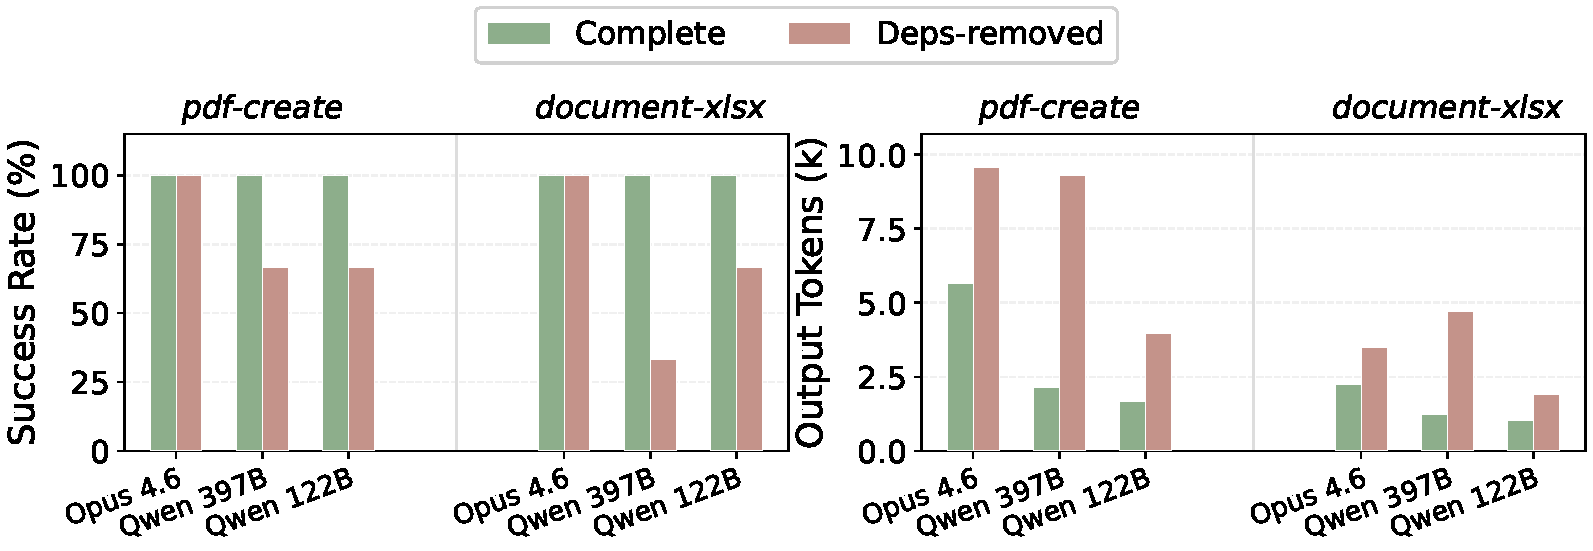
\includegraphics[width=\columnwidth]{figures/p3_env_binding_motivation.pdf}
  \caption{移除一项必要依赖会同时损害正确性与效率。}
  \label{fig:p3_env_motivation}
\end{figure}

\subsection{挑战}
\label{sec:insight:challenges}

技能以纯 Markdown 形式分发，使任何代理都能在无专用工具的情况下加载它们。
上述错配破坏了这一可移植性承诺。
恢复可移植性需要针对每个目标端适配技能，而这面临两个挑战。

\heading{C1：目标端在多个维度上不同。}
上述模型、代理框架与环境三个维度彼此独立变化。
一个需要沿某个维度进行适配的技能，在两个维度共同变化时可能需要另一种适配。
对于运行在功能丰富框架上的弱模型，正确修复方式不同于同一模型运行在最小框架上的修复方式。
这种交互使适配空间呈组合式增长：一套固定重写规则无法覆盖它。

\heading{C2：技能是非结构化自然语言。}
源代码在目标系统上运行前需要编译，并且具有可供工具分析的语法、类型和明确定义的 AST~\cite{aho2006compilers}。
相比之下，技能以自然语言编写。
尽管技能大多遵循共同惯例创建，不同技能在结构、术语和细节层次上仍有很大差异。
在进行任何适配前，都必须先从文本中恢复技能的隐式需求与工作流结构。
